
%-----------------------------------------------------------------------------------
%-----------------------------------------------------------------------------------
%                                      PREAMBLE
%-----------------------------------------------------------------------------------
%-----------------------------------------------------------------------------------
\documentclass{article}
%-----------------------------------------------------------------------------------
% GENERIC PACKAGES
\usepackage[utf8]{inputenc}
\usepackage{amsmath}
\usepackage{graphicx}
\usepackage{hyperref}
\usepackage{setspace}
\usepackage[T1]{fontenc}
\usepackage{multicol}
\usepackage{caption}
\usepackage{textcomp}
\usepackage{blindtext}
\usepackage{layouts}
\usepackage{float}

\newenvironment{Figure}
  {\par\medskip\noindent\minipage{\linewidth}}
  {\endminipage\par\medskip}
%-----------------------------------------------------------------------------------
% GEOMETRY
\usepackage{geometry}
\geometry{
    left=25mm,
    right=25mm,
    top=25mm,
    bottom=25mm
    }
\onehalfspacing
%-----------------------------------------------------------------------------------
% ACRONYMS
\usepackage{acro}
\DeclareAcronym{hri}{
  short=HRI,
  long=Human-Robot Interaction,
}
\DeclareAcronym{mis}{
  short=MIS,
  long=minimally Invasive Surgery,
}
\DeclareAcronym{ramis}{
  short=RAMIS,
  long=Robot-Assisted Minimally Invasive Surgery,
}
\DeclareAcronym{vf}{
  short=VF,
  long=Virtual Fixture,
}
\DeclareAcronym{psm}{
  short=PSM,
  long=Patient-Side Manipulator,
}
\DeclareAcronym{mtm}{
  short=MTM,
  long=Master Tool Manipulator,
}
\DeclareAcronym{hrsv}{
  short=HRSV,
  long=High-Resolution Stereo Viewer,
}
\DeclareAcronym{ecm}{
  short=ECM,
  long=Endoscope Camera Manipulator,
}

%-----------------------------------------------------------------------------------
% NEWCOMMANDS AND RENEWCOMMANDS
\newcommand{\cright}{\textsuperscript{\textregistered}\phantom{..}}
\newcommand{\vect}[1]{\textbf{#1}}
\newcommand{\fcaption}[1]{\captionof{figure}{\textit{\small #1}}}

%-----------------------------------------------------------------------------------

% TITLE
\title{
\begin{figure}[h!]
\centering

\includegraphics[width=0.5\textwidth]{images/logo_polimi_scritta2.eps}
\end{figure}
\textbf{Implementation and assessment of Assistance-as-Needed Virtual Fixtures for Surgical Training with a \textit{daVinci} surgical robot: an experimental study}
\\
\vspace{0.5cm}\large{\textit{Politecnico di Milano - Master of Science in Biomedical Engineering}}
\\
\vspace{0.5cm}\textit{\small{Academic year 2022/2023}}\vspace{0.5cm}\\
{\large \textbf{Candidate: \textit{Alberto Rota}}\\
\textbf{Supervisor: \textit{prof. Elena De Momi}}}}
\author{}
\date{}

%-----------------------------------------------------------------------------------
%-----------------------------------------------------------------------------------
%                                      BODY
%-----------------------------------------------------------------------------------
%-----------------------------------------------------------------------------------
\begin{document}
% TITLE
\maketitle
%-----------------------------------------------------------------------------------
% AUTHOR

% \vspace{1cm}
\begin{multicols}{2}

%-----------------------------------------------------------------------------------

\section{Introduction}
Since the introduction of \ac{ramis} in the healthcare market, patients have benefited from the diminishing of postoperative complications and an increase in the safety of procedures, while surgeons have been empowered by sophisticated robotic systems allowing the execution of complex tasks in adverse contexts. 

Surgical teams have been joined by robotic systems because of the number of benefits that result from the collaborative effort of the surgeon and the robot, combining the know-how and adaptation skills of the former and the high accuracy and stability of the latter. Such a synergistic perspective highlights the role of the \ac{hri} paradigm, which involves all aspects of understanding, designing, and evaluating robotic systems for use by or with humans \cite{Goodrich2007}. Most of the surgical robotics solutions on the market consist of a teleoperation console that interfaces with the practicioner and, separate from it, the surgical robot itself, which mimics the movements of the surgeon in real-time. This setup allows for higher motion accuracy, tremor filtration and magnified viewing of the surgical area; nonetheless tactile forces, friction and texture perception are excluded from the so crucial visuo-haptic feedback loop that would guide the surgeon in a standard "non-robotic" procedure.

This work, specifically, studies and evaluates the role of Virtual Fixtures in the context of surgical training. \acp{vf} are high-level control strategies employed for assisting humans in man-machine collaboration tasks \cite{Bowyer2014}. In the context of surgical robotics, \acp{vf} assist the surgeon by providing haptic guidance at the level of the "master" manipulator, generating mechanical forces and torques which re-direct the motion of the surgeon's hands. These assistance strategies may be most beneficial in the training process that aspiring surgeons undertake, which often takes place in a simulated virtual environment. Exploiting the customizability of simulated surgical tasks together with the implementation of \acp{vf} will enhance the process of learning key surgical skills, in terms of performance, retention and transfer.



\section{State of the art}
Surgical robotics companies usually commercialize a simulation framework in parallel to clinical robots. A survey of the most relevant training simulators on the market was conducted in \cite{Bric2016}, a review that also assesses the suitability of virtual environments as comparable to the one of dry-lab setups. However, since no commercially available clinical system implements a force-based assistive modality similar to the one of virtual fixtures, none of the training simulators employ \acp{vf} either. The role of such assistive strategies in a real surgical scenario is still uncertain and shall be assessed only through an extensive clinical trial, and as a matter of fact the vast majority of training protocols implementing \acp{vf} regards \textit{ad-hoc} systems like \cite{Lin2014}, which are limited both in terms of tasks implemented and in terms of evaluation protocols. Indeed, few studies \cite{Enayati2018} have evaluated the trainee's performance on multiple diverse tasks and over the course of multiple training days, and none has yet investigated the role of haptic assistance on skill retention and skill transfer. 

This work proposes an evaluation of the role of \acp{vf} in surgical training with a multi-day experimental protocol articulated in two phases, designed in order to highlight the difference in the transfer and retention of skills between a control group and an assisted group. 
\section{Materials and methods}
\subsection{Surgical Simulator}
This research was conducted on a \textit{daVinci}\cright surgical robot integrated with the open-source dVRK \cite{Kazanzidesf2014} framework. The \acp{mtm} of the \textit{daVinci}\cright are in fact equipped with motors usually employed for the sake of homing and calibration; the \ac{vf} forces and torques are generated by energizing these motors according to the inverse kinematics of the manipulators. A ROS \cite{ros} framework manages the communication between the teleoperation console of the dVRK and the virtual surgical scene, which is built upon the Unity\cright physics engine: therefore, the real \acp{psm} do not move during teleoperation, as the joint coordinates are communicated only to the virtual 3D objects.

\begin{figure*}
  \centering
      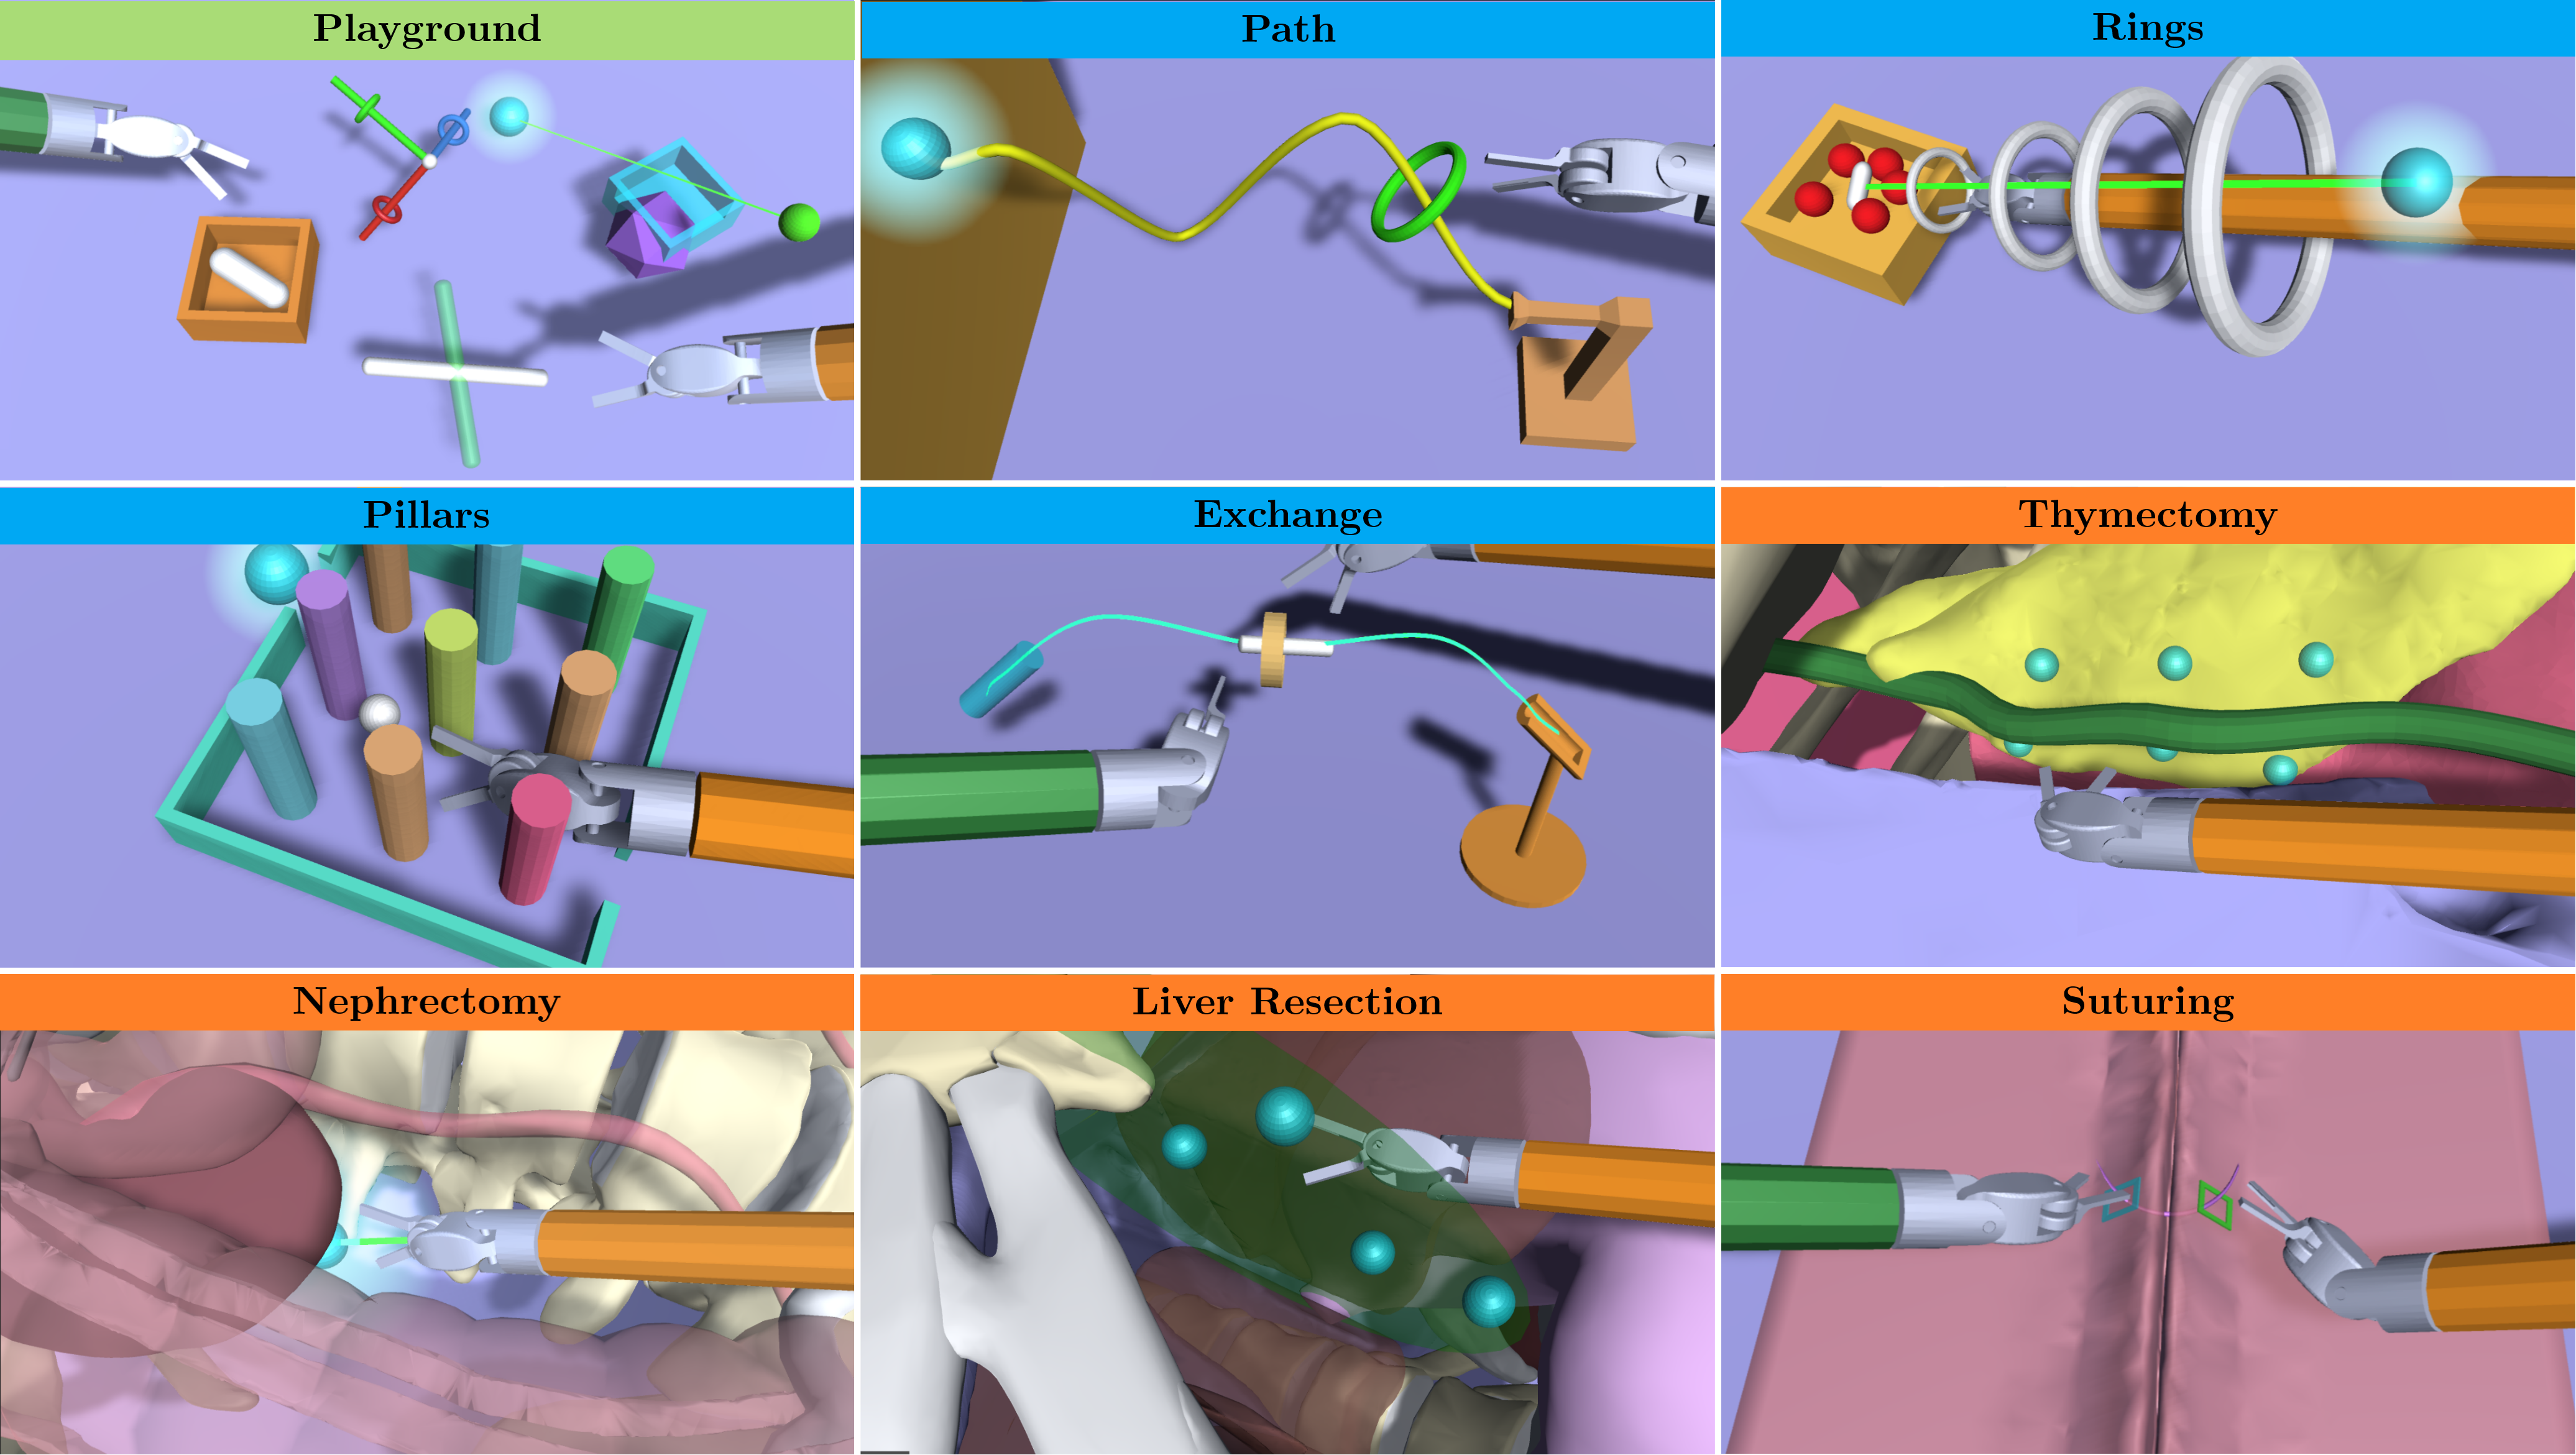
\includegraphics[width=\linewidth]{images/PANEL_named.png}
      \small{
      \caption{\textit{Snapshot of the simulated surgical tasks, with the respective denomination. Training tasks have blue headlines, while realistic evaluation tasks have orange headlines. \textit{Playground} is a propaedeutic task and isn't featured in the}}}
      \label{fig:taskspanel}
\end{figure*}

The simulator comprises eight surgical tasks, four of which (\textit{Path, Rings, Pillars} and \textit{Exchange}) are simplistic training tasks built with objects of simple geometry, while the remaining four (\textit{Liver Resection, Nephrectomy, Thymectomy} and \textit{Suturing}) emulate \textit{in-vivo} surgical procedures and are therefore more realistic. Fig.\ref{fig:taskspanel} collects snapshots of the tasks. All of these are constructed and set-up in order to be as challenging as possible in relation to a specific surgical skill. A set of fundamental pre-operative and intra-operative skills that any robotic surgeon should acquire during training was proposed in \cite{Smith2014}. Specifically:
\begin{itemize}
  \item \textit{Path} and \textit{Liver Resection} require articulate wrist motion and stability
  \item \textit{Rings} and \textit{Nephrectomy} survey the depth perception skills
  \item \textit{Pillars} and \textit{Thymectomy} are hand-eye coordination tasks
  \item \textit{Exchange} and \textit{Suturing}, both bi-manual tasks, challenge the capabilities in terms of instrument exchange 
\end{itemize}
Each training task having a corresponding emulated surgical procedure will allow, during the experimental phase, to evaluate the transferability of skills.

The simulator also exploits 3D viewing capability of the \ac{hrsv} installed on the teleoperation surgical console: two virtual cameras are positioned in the Unity\cright scene at a distance of 5.3mm, as their feed is sent separately on the left and right oculars at the console achieving a three-dimensional perception of the virtual environment.
\subsection{Virtual Fixtures}
During teleoperation the surgeon is de-coupled from the patient: this is necessary in order to exploit the benefits of a robotic solution, which requires the system to be "in between" the practitioner and the patient in order to enhance the surgical experience. However, this de-coupling removes the haptic component from the motion control feedback loop of the surgeon, who is used to relying on the sense of touch when operating with a conventional approach. For this reason, this work analyses how the introduction of haptics in a virtual surgical environment may enhance the training phase, acting as a guidance and error-correcting medium. 

In the context Virtual Fixtures, also known as Active Constraints, a haptic force is applied to the manipulators at the surgical console, which re-directs the motion of the surgeon's hands in case of improper or unsafe maneuvers. The magnitude and direction of the \acp{vf} force are computed from the \ac{psm} position and orientation relative to the surgical space and the position of objects in the scene, in a true feedback fashion. A transformation mapping the \ac{psm} operatory space to the \ac{mtm} console space is necessary in order to sensibly use the feedback force as a corrective strategy.

\begin{equation}
  \vect{f}_{MTM} = T_{PSM}^{MTM}\cdot \vect{f}_{PSM}
\end{equation}

\subsubsection{Distance Mapping}
Most of the assistance strategies implemented here will use the distance from the \ac{psm} to the target or obstacle as the primary metric for determining the intensity of the feedback force or torque. However, different surgical tasks and situations require a level of control over how the distance is taken into account, and for this reason a sigmoidal mapping function was employed for the normalization of the linear or angular error into a suitable interval. Specifically, such mapping is formulated as:
\begin{equation}
  f_{map}(x) = \frac{1}{1+e^{\frac{\delta\cdot w(x-t-h)}{0.2}}}
  \label{eq:sigmoidalmap}
\end{equation}
with $\delta = +1$ for guidance \acp{vf} and $\delta = -1$ for avoidance \acp{vf}. Here:
\begin{itemize}
  \item $t$ is the fixture \textit{threshold}, hence the value at which the sigmoid starts to significantly increase from zero
  \item $h$ is the distance from the threshold at which \textit{half} of the maximum force is provided
  \item $w$ controls the \textit{width} of the linear region, hence the steepness of the curve 
\end{itemize}
For example, if $t=2$mm and $h=3$mm the surgeon will start to feel a force for errors higher than 2mm, and at 5mm he/she will half of the maximum force delievered.

\begin{Figure}
  \centering
      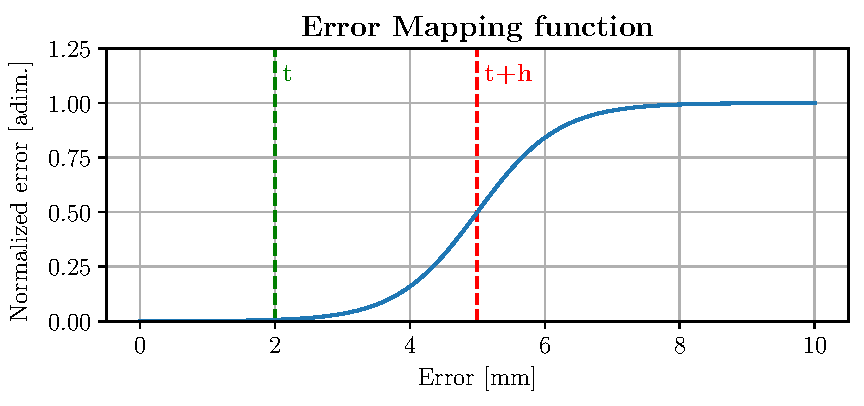
\includegraphics[width=\linewidth]{images/mappingfunction.eps}
      \fcaption{Plot of the Error Mapping function. The position of$t$ and $t+h$ can be set manually to achieve a suitable behavior of the assistance strategy}
      \label{fig:mappingfunctiion}
\end{Figure}

\subsubsection{Trajectory Guidance}
A \textit{Trajectory Guidance Virtual Fixture} aids the surgeon in following a reference trajectory and maintaining the correct orientation of the surgical tool. For this \ac{vf}, the feedback force is computed as the sum of a viscous and an elastic contribution, weighted by the parameters $k$ and $\eta$ respectively.
\begin{equation}
    \vect{f} = k \cdot \vect{d} + \eta \cdot
    \begin{cases} 
        \vect{d}, & \textit{if         } \vect{v}\cdot\vect{d}<0 \\
         rotate(\vect{v},\theta,\vect{r}), & \textit{otherwise}
    \end{cases}
    \label{eq:trajVFforce}
\end{equation} 


\begin{equation}
  \vect{T} = k \cdot acos (\vect{z}\cdot\vect{t} ) \cdot \vect{z} \times \vect{t} + \eta \cdot acos (\vect{z}\cdot\vect{t} ) \cdot \vect{z} \times \vect{t}
    \label{eq:trajVFtorque}
  \end{equation}
with $\theta = (1+\vect{v}\cdot\vect{d})\cdot\frac{\pi}{2}$ and $\vect{r} = \vect{v}\times\vect{d}$ the angle and axis of rotation respectively

\subsubsection{Insertion Guidance}
\subsubsection{Obstacle Avoidance}
\subsubsection{Surface Guidance}

\subsection{Clinical Validation}
Two resident surgeons from the \textit{Istituto Europeo di Oncologia}, both regularly performing \ac{ramis} procedures with the \textit{daVinci}\cright robot, kindly dedicated their time in testing the surgical simulator in all its aspects, from the motion truthfulness to the complexity of the wrist articulation to the invasiveness and visco-elastic balance of the virtual fixtures. Their opinion and expertise were precious and insightful tools that guided the development towards a clinically validated robotic surgical simulator. 

\subsection{Experimental Protocol}
The effectiveness of the haptic virtual fixture paradigm has been assessed with an experimental study where the performance of un-assisted subjects in a control group was compared to the one recorded from subject to whom was provided haptic assistance. Since the aim of this work is to establish the role of \acp{vf} in the training context, eight novice subjects with little to no experience with surgical robotics were recruited for the study. Subjects were 25\% females and 75\% males, between 23 and 27 years of age, all right-handed and either had never teleoperated a surgical robot or did it less than 5 times. Assignation to the control or assisted group was random.

The subjects underwent a week-long training phase:
\begin{itemize}
  \item On \textit{Day 1}, they were given a concise explanation about the \textit{daVinci}\cright surgical system, the simulator, haptics, and the training protocol. Later, each subject experienced 5 minutes in a \textit{Playground} environment, purposely designed to understand the elementary mechanics of teleoperation, clutching and object grasping. No performance metric was recorded at this time
  \item From \textit{Day 2} to \textit{Day 5} they were asked to execute the four training tasks of the simulator (\textit{Path, Rings, Pillars} and \textit{Exchange}), each one for a total of 3 repetitions. Tasks appeared sequentially in a random order, contributing to un-bias the results. At the beginning of each daily session, subjects could interact with the \textit{Playground} task for 1 minute at maximum.
  \item On \textit{Day 6} and \textit{Day 7} subjects were given a break period and no training was performed
  \item On \textit{Day 8} they were asked to execute the four validation tasks of the simulator (\textit{Thymectomy, Nephrectomy, Liver Resection} and \textit{Suturing}), each one for a total of 3 repetitions. Again, tasks appeared sequentially in a random order, contributing to un-bias the results.
\end{itemize}

\subsection{Metrics}


\section{Results}
\section{Discussion}
\section{Conclusions}
%-----------------------------------------------------------------------------------
% BIBLIOGRAPHY
\bibliographystyle{unsrt}
\bibliography{refs.bib}
%-----------------------------------------------------------------------------------
\end{multicols}
\end{document}



